

\subsection{Model Comparison}

We begin with the classical Ordinary Least Squares (OLS) regression model,
specified as
\begin{equation}
	y_i = \alpha + \sum_{j=1}^{p} x_{ij}\beta_j + \epsilon_i,
	\label{eq:OLS}
\end{equation}
where the error terms are assumed to be independently and identically
distributed.

To account for spatial dependence, a spatial weights matrix $W$ is incorporated
into the regression framework. One such specification is the Spatial Durbin
Model (SDM), given by
\begin{equation}
	y = X\beta + \rho WX + \epsilon,
	\label{eq:SDM}
\end{equation}
which expands to
\begin{equation}
	y_{it}
	=
	\alpha
	+ \sum_{j=1}^{p} x_{it,j}\beta_j
	+ \rho \sum_{k=1}^{N} w_{ik} x_{kt}
	+ \epsilon_{it}.
	\label{eq:SDM_exp}
\end{equation}

Alternative spatial specifications incorporate spatial dependence directly into
the response variable, as in the Spatial Autoregressive (SAR) model,
\begin{equation}
	y = \alpha + X\beta + \rho WY + \epsilon,
	\label{eq:SAR}
\end{equation}
or into the error structure, as in the Spatial Error Model (SEM),
\begin{equation}
	\begin{split}
		y & = \alpha + X\beta + u,  \\
		u & = \gamma Wu + \epsilon.
	\end{split}
	\label{eq:SEM}
\end{equation}

As an alternative to parametric spatial regression, we consider a
semi-parametric specification that incorporates spatial dependence through a
smooth function of location:
\begin{equation}
	y = \alpha + \sum_{j=1}^{p} x_{it,j}\beta_j + f(C_i) + \epsilon,
	\label{eq:tensor}
\end{equation}
where $C_i$ denotes the centroid coordinates of observation $i$, and
$f(C_i)$ is a spatial smoothing function constructed using tensor-product
splines.

We hypothesize that the semi-parametric model may outperform parametric spatial
regression models when the true spatial weights matrix $W$ is unknown or
misspecified, particularly in terms of predictive accuracy and robustness.
\subsection{Spatial Smoother}

As previously noted, the term $f(C_i)$ represents a penalized spatial smoother
used as an alternative to specifying a spatial weights matrix in order to
account for spatial correlation. Beginning with a univariate basis expansion,
any smooth function of a single covariate can be expressed as a linear
combination of spline basis functions. In particular, a cubic spline
representation may be written as
\begin{equation}
	f(x) = \sum_{j=1}^{k} b_j(x)\,\beta_j.
\end{equation}

This representation generates a smooth curve constructed from a set of local
basis functions, as illustrated in Figure~\ref{fig:bsplines}.

\begin{figure}[H]
	\centering
	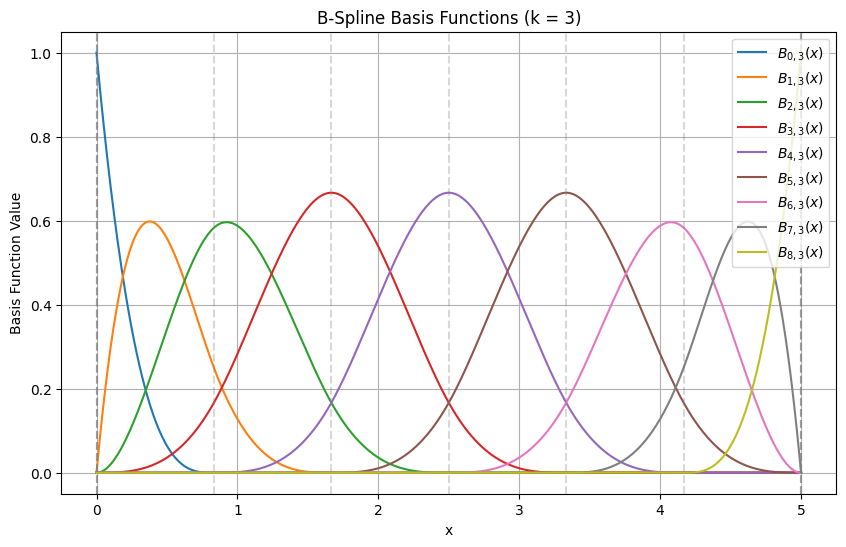
\includegraphics[width=0.4\textwidth]{assets/b-splines.png}
	\caption{Basis spline functions}
	\label{fig:bsplines}
\end{figure}

To extend this framework to multiple variables, a separate basis expansion is
first specified for each covariate. For two variables $x$ and $z$, these
expansions take the form
\[
	f_x(x) = \sum_{j=1}^{k} b_j(x)\,\beta_j,
	\qquad
	f_z(z) = \sum_{j=1}^{k} d_j(z)\,\delta_j.
\]

The coefficients of the basis functions in one dimension may then be allowed to
vary smoothly as a function of the other variable. Specifically, letting the
coefficients $\beta_j$ vary smoothly with respect to $z$ yields
\[
	\beta_j(z) = \sum_{l=1}^{L} \delta_{jl} d_l(z).
\]

Substituting this expression into the original basis expansion produces the
tensor–product smoother
\begin{equation}
	f_{xz}(x,z)
	=
	\sum_{j=1}^{k}
	\sum_{l=1}^{L}
	\delta_{jl}\,
	b_j(x)\, d_l(z).
\end{equation}

Implementing this construction results in a smooth surface over the joint
domain of $(x,z)$, as illustrated in Figure~\ref{fig:tensor}.

\begin{figure}[H]
	\centering
	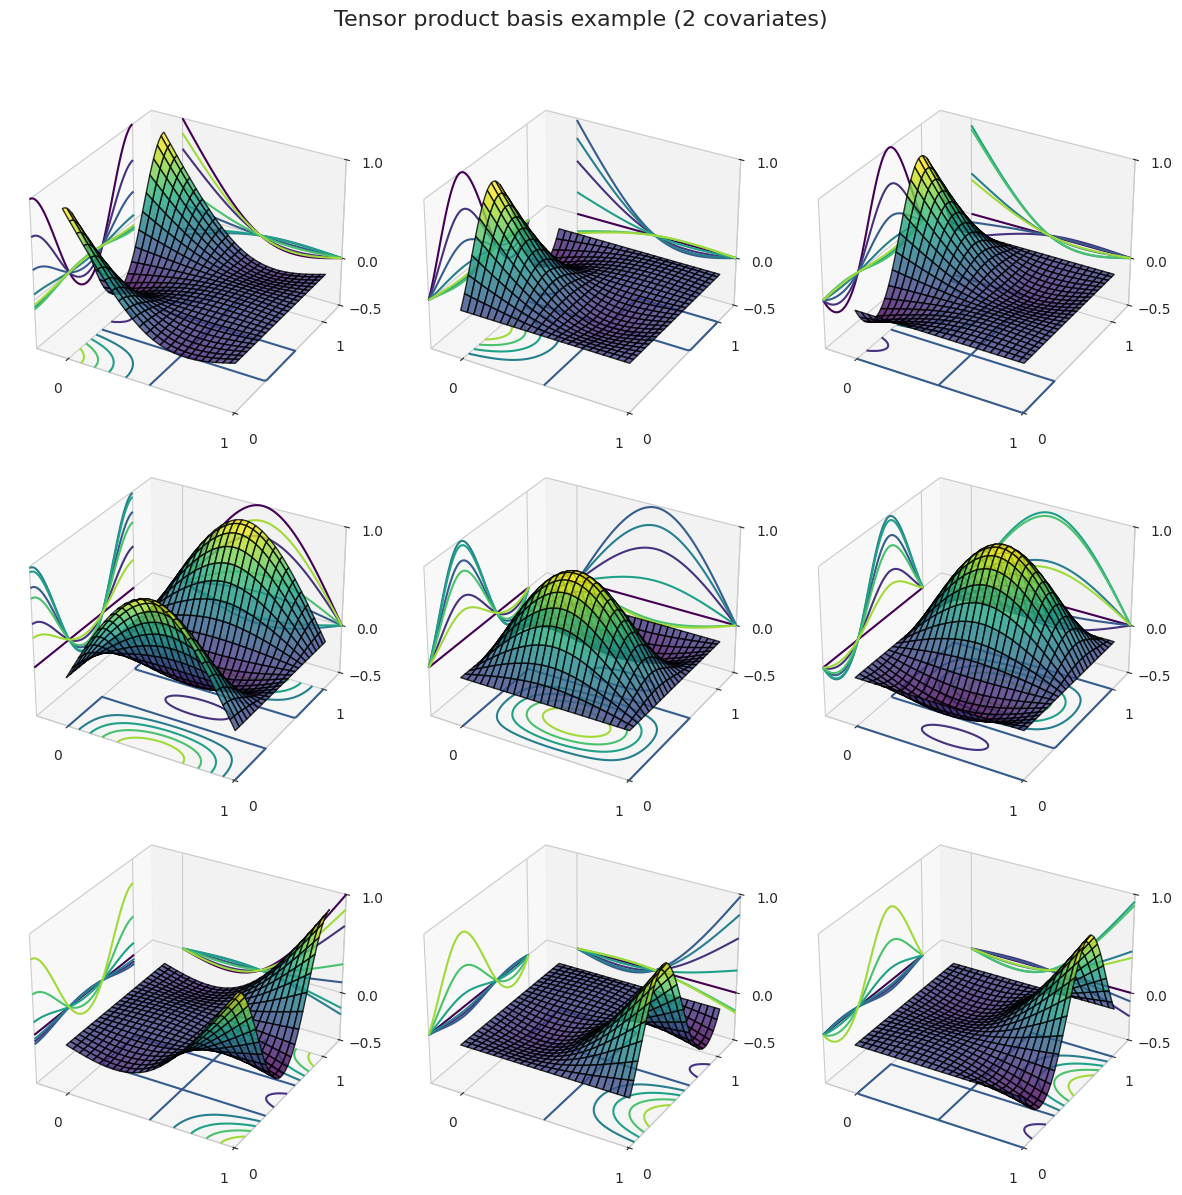
\includegraphics[width=0.4\textwidth]{assets/tensor.png}
	\caption{Tensor-product spline surface}
	\label{fig:tensor}
\end{figure}

The tensor–product smoother can be expressed compactly using the tensor
(Kronecker) product design matrix
\[
	X_{\text{tensor}} = B \otimes D,
\]
where $B$ denotes the spline basis matrix for $x$ and $D$ denotes the spline
basis matrix for $z$.

Estimation of the smoother coefficients is carried out by solving the
ridge–regularized least-squares problem
\[
	\min_{\delta}
	\; \| y - X_{\text{tensor}} \delta \|_2^2
	\;+\;
	\alpha \, \| \delta \|_2^2,
\]
where the penalty parameter $\alpha$ controls the smoothness of the estimated
surface.


\subsection{Cobb--Douglas Interpretation}

Incorporating a tensor-product spatial smoother into the Cobb--Douglas production
function yields the following specification:
\begin{equation}
	Y_{it}
	=
	K_{it}^{\alpha}
	L_{it}^{\beta}
	\exp\{ f(\text{lat}_i, \text{lon}_i) + \gamma_t + \epsilon_{it} \},
	\label{eq:Cobb tensor}
\end{equation}

This equation serves as the primary model employed in this research. The parametric
components preserve the standard Cobb--Douglas interpretation of output elasticities
with respect to capital and labor, while the tensor-product function $f(\text{lat}_i,
	\text{lon}_i)$ flexibly captures spatial variation in productivity. By modeling spatial
effects nonparametrically, this approach avoids the need to specify a spatial weights
matrix and aims to produce more reliable and robust parameter estimates in the presence
of unknown or complex spatial dependence.

\subsection{Data Sources and Variable Specification}

To apply the proposed models to the Puerto Rican economy, we utilize high-frequency sub-national data. Given the lack of official municipal-level GDP reports in real-time, the following proxies and data sources are employed:

\begin{itemize}
	\item \textbf{Output ($Y$):} Following established econometric literature that uses electricity consumption as a high-correlation proxy for economic activity, we utilize municipal energy consumption data provided by \textbf{LUMA Energy}. This allows for a more granular temporal analysis than traditional annual proxies.

	\item \textbf{Capital ($K$):} Physical capital stocks are derived from the \textbf{Centro de Recaudación de Ingresos Municipales (CRIM)}. Specifically, data is extracted from the \textit{Personal Property Tax Return (Planilla de Contribución sobre la Propiedad Mueble AS-29.1)}. Key indicators include:
	      \begin{itemize}
		      \item \textbf{Current Assets:} Inventory, materials, and supplies (Encasillado C).
		      \item \textbf{Fixed Assets:} Machinery, equipment, and leasehold improvements.
	      \end{itemize}

	\item \textbf{Labor ($L$):} Labor input is measured using employment and wage data from the \textbf{Quarterly Census of Employment and Wages (QCEW)}. This dataset provides a comprehensive count of establishments, employment, and wages for workers covered by State unemployment insurance laws, categorized by North American Industry Classification System (NAICS) codes.
\end{itemize}

The integration of these datasets provides a panel structure desegregated by municipality ($i$) and time ($t$), which is essential for the spatial and semi-parametric models described in Equations \ref{eq:SAR} and \ref{eq:tensor}.
